\documentclass[12pt]{report}

\usepackage{cmap}
\usepackage[T2A]{fontenc}
\usepackage[utf8]{inputenc}
\usepackage[english,russian]{babel}

\usepackage{amssymb}

\usepackage{longtable}

\usepackage{graphicx}
\usepackage{float}%"Плавающие" картинки
\usepackage{wrapfig}%Обтекание фигур (таблиц, картинок и прочего)
\graphicspath{{images/}}
\usepackage[usenames]{color}

\usepackage{listings}

\lstset{
language=haskell,                 % выбор языка для подсветки (здесь это С)
basicstyle=\small\sffamily, % размер и начертание шрифта для подсветки кода
numbers=left,               % где поставить нумерацию строк (слева\справа)
numberstyle=\tiny,           % размер шрифта для номеров строк
stepnumber=1,                   % размер шага между двумя номерами строк
numbersep=5pt,                % как далеко отстоят номера строк от подсвечиваемого кода
showspaces=false,            % показывать или нет пробелы специальными отступами
showstringspaces=false,      % показывать или нет пробелы в строках
showtabs=false,             % показывать или нет табуляцию в строках
frame=single,              % рисовать рамку вокруг кода
tabsize=1,                 % размер табуляции по умолчанию равен 2 пробелам
captionpos=t,              % позиция заголовка вверху [t] или внизу [b] 
breaklines=true,           % автоматически переносить строки (да\нет)
breakatwhitespace=false, % переносить строки только если есть пробел
escapeinside={\#*}{*)}   % если нужно добавить комментарии в коде
}


% Для измененных титулов глав:
\usepackage{titlesec, blindtext, color} % подключаем нужные пакеты
\definecolor{gray75}{gray}{0.75} % определяем цвет
\newcommand{\hsp}{\hspace{20pt}} % длина линии в 20pt
% titleformat определяет стиль
\titleformat{\chapter}[hang]{\Huge\bfseries}{\thechapter\hsp\textcolor{gray75}{|}\hsp}{0pt}{\Huge\bfseries}


\usepackage{pgfplots}
\usepackage{filecontents}
\usetikzlibrary{datavisualization}
\usetikzlibrary{datavisualization.formats.functions}


\begin{filecontents}{DamLevT.dat}
	3 0.00666
	4 0.01661
	5 0.01867
\end{filecontents}

\begin{filecontents}{DamLevR.dat}
	3 0.05122
	4 0.21172
	5 0.82129
\end{filecontents}



\begin{filecontents}{LevT.dat}
	10 0.05143
	20 0.17495
	30 0.37773
	40 0.75407
	60 2.40581
	80 5.97663
	100 12.90033
\end{filecontents}

\begin{filecontents}{DamLevT2.dat}
	10 0.07763
	20 0.25776
	30 0.5983
	40 1.39289
	60 4.85997
	80 13.00983
	100 24.0279
\end{filecontents}


\begin{document}
	\begin{titlepage}
		\centering
		{\scshape\LARGE МГТУ им. Баумана \par}
		\vspace{3cm}
		{\scshape\Large Лабораторная работа №1\par}
		\vspace{0.5cm}	
		{\scshape\Large По курсу: "Анализ алгоритмов"\par}
		\vspace{1.5cm}
		{\huge\bfseries Расстояние Левенштейна\par}
		\vspace{2cm}
		{\Large Работу выполнил: Левушкин Илья, ИУ7-52Б\par}
		\vspace{0.5cm}
		{\Large Преподаватели:  Волкова Л.Л., Строганов Ю.В.\par}
		
		\vfill
		\large \textit {Москва, 2019} \par
	\end{titlepage}

    \tableofcontents
    
    \newpage
    \chapter*{Введение}
    
    \addcontentsline{toc}{chapter}{Введение}
    
    \textbf{Алгоритмы нечеткого поиска} (также известного как поиск по сходству или fuzzy string search) являются основой систем проверки орфографии и полноценных поисковых систем вроде Google или Yandex, а также применяются в биоинформатике для сравнения генов, хромосом и белков. Например, такие алгоритмы используются для функций наподобие «Возможно вы имели в виду …» в тех же поисковых системах ~\cite{Algorithms}.
    \vspace{0.5cm}
    
    Нечеткий поиск является крайне полезной функцией любой поисковой системы. Вместе с тем, его эффективная реализация намного сложнее, чем реализация простого поиска по точному совпадению.
    \vspace{0.5cm}
    
    Задачу нечеткого поиска можно сформулировать так:
    «По заданному слову найти в тексте или словаре размера n все слова, совпадающие с этим словом (или начинающиеся с этого слова) с учетом k возможных различий».
    \vspace{0.5cm}
    
    Например, при запросе «Машина» с учетом двух возможных ошибок, найти слова «Машинка», «Махина», «Малина», «Калина» и так далее.
    \vspace{0.5cm}
    
    Алгоритмы нечеткого поиска характеризуются метрикой — функцией расстояния между двумя словами, позволяющей оценить степень их сходства в данном контексте. Строгое математическое определение метрики включает в себя необходимость соответствия условию неравенства треугольника (X — множество слов, p — метрика):
    \vspace{0.5cm}
    
    \begin{equation} \label{eq0}
    \rho (x, y) \leqslant \rho (x, z) + \rho (z, y), \;\;\; x, y, z \in X
    \end{equation}
    \vspace{0.5cm}
    
    Между тем, в большинстве случаев под метрикой подразумевается более общее понятие, не требующее выполнения такого условия, это понятие можно также назвать расстоянием.
    \vspace{0.5cm}
    
    В числе наиболее известных метрик — расстояния Хемминга, Левенштейна и Дамерау-Левенштейна. При этом расстояние Хемминга является метрикой только на множестве слов одинаковой длины, что сильно ограничивает область его применения.
    \vspace{0.5cm}
    
    Впрочем, на практике расстояние Хемминга оказывается практически бесполезным, уступая более естественным с точки зрения человека метрикам. Поэтому больший интерес для изучения представляет собой алгоритм Левенштейна, а также его модификация - Дамерау-Левенштейна, который учитывает распространенную ошибку человека при наборе слов: "Персетановка билз лежаищх бкув в солве месатми"
    
   
    
    
    \chapter{Аналитическая часть}
    
    
    \section{Цель} 
    Целью данной лабораторной работы является изучение алгоритмов Левенштейна и Дамерау-Левенштейна.
    
    \section{Задачи}
    Для достижения поставленной цели необходимо решить следующие {\bf задачи}:
    
    
    \begin{itemize}
    	\item проанализировать и разработать существующие реализации алгоритмов Левенштейна и Дамерау-Левенштейна;
    	\item выбрать технологии для последующих реализаций и иследования
    	алгоритмов;
    	\item реализовать эти алгоритмы;
    	\item произвести тестирование корректности работы реализаций;
    	\item сравнить быстродействие реализаций;
    	\item описать и обосновать полученные результаты в отчете о выполненной лабораторной работе, выполненного как расчётно-пояснительная
    	записка к работе.
    \end{itemize}
    
    
    \newpage
    \section{Алгоритмы Левенштейна и Дамерау-Левенштейна}
    
    Задача по нахождению расстояния Левенштейна заключается в поиске минимального количества операций вставки/удаления/замены для превращения одной строки в другую.
    
    При нахождении расстояния Дамерау — Левенштейна добавляется операция транспозиции (перестановки соседних символов).  
    
    \textbf{Действия обозначаются так:} 
    \begin{enumerate}
    	\item D (англ. delete) — удалить,
    	\item I (англ. insert) — вставить,
    	\item R (replace) — заменить,
    	\item M (match) - совпадение.
    \end{enumerate}
    
    Пусть $S_{1}$ и $S_{2}$ — две строки (длиной M и N соответственно) над некоторым алфавитом, тогда расстояние Левенштейна можно подсчитать по следующей рекуррентной формуле:
    
    \begin{equation} \label{eq1}
    D(i,j) = \left\{ \begin{array}{ll}
    0, & \textrm{$i = 0, j = 0$}\\
    i, & \textrm{$j = 0, i > 0$}\\
    j, & \textrm{$i = 0, j > 0$}\\
    min(\\
    D(i,j-1)+1,\\
    D(i-1, j) +1, &\textrm{$j>0, i>0$}\\
    D(i-1, j-1) + m(S_{1}[i], S_{2}[j])\\
    ),
    \end{array} \right.
    \end{equation}
    
    где $m(a,b)$ равна нулю, если $a=b$ и единице в противном случае; $min\{\,a,b,c\}$ возвращает наименьший из аргументов ~\cite{leven}, ~\cite{recurs}.
    
    Расстояние Дамерау-Левенштейна вычисляется по следующей рекуррентной формуле:
    \begin{equation} \label{eq2}
    D(i,j) = \left\{ \begin{array}{ll}
    0, & \textrm{$i = 0, j = 0$}\\
    i, & \textrm{$j = 0, i > 0$}\\
    j, & \textrm{$i = 0, j > 0$}\\
    min(\\
    D(i,j-1)+1,\\
    D(i-1, j) +1, &\textrm{$j>0, i>0$}\\
    D(i-1, j-1) + m(S_{1}[i], S_{2}[j])\\
    D(i-2, j-2) + 1, &\textrm{if $i,j>1$ and $a_{i} = b_{j-1},a_{i-1}=b_{j} $}\\
    )
    &\textrm otherwise\\
    min(\\
    D(i,j-1)+1,\\
    D(i-1, j) +1, &\textrm{$j>0, i>0$}\\
    D(i-1, j-1) + m(S_{1}[i], S_{2}[j])\\
    )
    \end{array} \right.
    \end{equation}
    ~\cite{damerau}
    \vspace{0.5cm}
    
    
    
    \section{Выводы}
		В рамках данной работы были выбраны для исследования алгоритмы Левенштейна и Дамерау-Левенштейна.
    	Математическое описание обоих алгоритмов приведено в формулах \ref{eq1}, \ref{eq2}
    
    
    
    \chapter{Конструкторская часть}
    
    \section{Способы реализаций алгоритмов}
    Алгоритмы Левенштейна и Дамерау-Левенштейна могут быть реализованы следущими способами:
    \begin{itemize}
    	\item рекурсивный метод;
    	\item матричный метод.
    \end{itemize}


    Первый представляет собой рекурсивное вычисление всех расстояний между словами, и выбором минимального из полученных решений.
    
    Сами рекурсии работ алгоритмов задаются следующим образом:
    \vspace{0.5cm}
    
    {\bf Обозначения:}
    \begin{itemize}
    	\item str1, str2 - Строки
    	\item p - Расстояние
    	\item length - Длина Строки
    	\item str[length - 1] - Строка без первого элемента слева
    	\item == - Проверка на равенство
    \end{itemize}
    \vspace{0.5cm}
    
    {\bf Рекурсия алгоритма Левенштейна}
   	
    На входе: str1, str2
    \begin{itemize}
    	\item При первом вызове рекурсии расстояние p = 0
    	\item Если длина одной из строк стала равна 0, то к полученному ранее расстоянию p добавляется длина другой строки.  (см. формулу \ref{eq1})
    	\item В случае, если длины обоих строк равны 0, то к полученному ранее расстоянию p ничего не добавляется.
    	\item Вызов рекурсий со следующими параметрами:
    	\begin{itemize}
    		\item $str1[length - 1]$, $str2$, $p + 1$
    		\item $str1$, $str2[length - 1]$, $p + 1$
    		\item $str1[length - 1]$, $str2[length - 1]$, $p + $ если $str1[1] == str2[1]$, то 0, иначе 1
    	\end{itemize}
    \end{itemize}

	{\bf Рекурсия алгоритма Дамерау-Левенштейна}
	
	На входе: str1, str2, p
	\begin{itemize}
		\item При первом вызове рекурсии p = 0
		\item Если длина одной из строк стала равна 0, то к полученному ранее расстоянию p добавляется длина другой строки.  (см. формулу \ref{eq1})
		\item В случае, если длины обоих строк равны 0, то к полученному ранее расстоянию p ничего не добавляется.
		\item Вызов рекурсий со следующими параметрами:
		\begin{itemize}
			\item $str1[length - 1]$, $str2$, $p + 1$
			\item $str1$, $str2[length - 1]$, $p + 1$
			\item $str1[length - 1]$, $str2[length - 1]$, $p + $если $str1[1] == str2[1]$, то 0, иначе 1
			\item если $str1[1] == str2[2]$ и $str1[2] == str1[1]$, то $str1[length - 2]$, $str2[length - 2]$, $p + 1$, иначе не вызывать рекурсию.
		\end{itemize}
	\end{itemize}

    Полученные "листья дерева" и будут являться решениями.
    \newpage
    
    {\bf Матричная реализация алгоритмов}
    Матричная реализация алгоритмов редставляет собой нахождение матрицы наименьших расстояний слов:
    
    \begin{equation}
    \left(
     \begin{array}{cccc}
    	p(str1[1], str2[1]) & p(str1[1, 2], str2[1]) & \ldots & p(str[length], str2[1])\\
    	p(str1[1], str2[1,2]) & p(str1[1, 2], str2[1,2]) & \ldots & p(str[length], str2[1,2])\\
    	\vdots & \vdots & \ddots & \vdots\\
    	p(str1[1], str2[]length]) & p(str1[1, 2], str2[length] & \ldots & p(str[length], str2[length])
    \end{array}
    \right)
    \end{equation}
    Где последнее расстояние слов $(str1[length], str2[length])$ и будет являться решением.
    
    Каждая элемент матрицы находится по следующим правилам:
    
    {\bf Алгоритм Левенштейна}
    \begin{equation}
    p[i][j] = min(p[i-1][j] + 1, p[i][j-1] + 1, p[i-1][j-1]+k)
    \end{equation}
    Где $k = 0$, если $str1[i] == str2[j]$, иначе $k = 1$
    
    
    {\bf Алгоритм Дамерау-Левенштейна}
    
    \begin{equation}
    p[i][j] = min(p[i-1][j] + 1, p[i][j-1] + 1, p[i-1][j-1]+k, p[i-2][j-2] + f)
    \end{equation}
    Где $k = 0$, если $str1[i] == str2[j]$, иначе $k = 1$
    
    $f = 1$, если $str1[i] == str2[j-1] \& str1[i-1] == str2[j]$, иначе $f = 2$
    \vspace{0.5cm}
    
    
   \section{Схемы алгоритмов}
   \newpage
   На рисунках ~\ref{ris:image1}, ~\ref{ris:image2}, ~\ref{ris:image3}, ~\ref{ris:image4}, ~\ref{ris:image5}, ~\ref{ris:image6}, ~\ref{ris:image7} представлены схемы реализаций алгоритмов Левенштейна и Дамерау-Левенштейна.
   
   \begin{figure}[h!]
   	\centering
   	\begin{minipage}[h!]{0.49\linewidth}
   		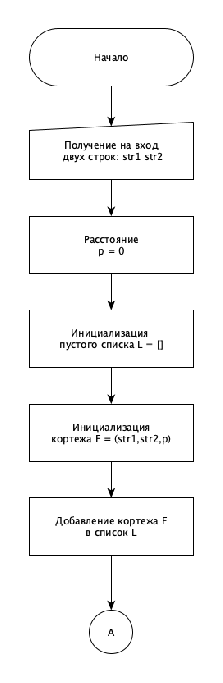
\includegraphics[width=0.5\linewidth]{LevenR}
   	\end{minipage}
   \begin{minipage}[h!]{0.49\linewidth}
   		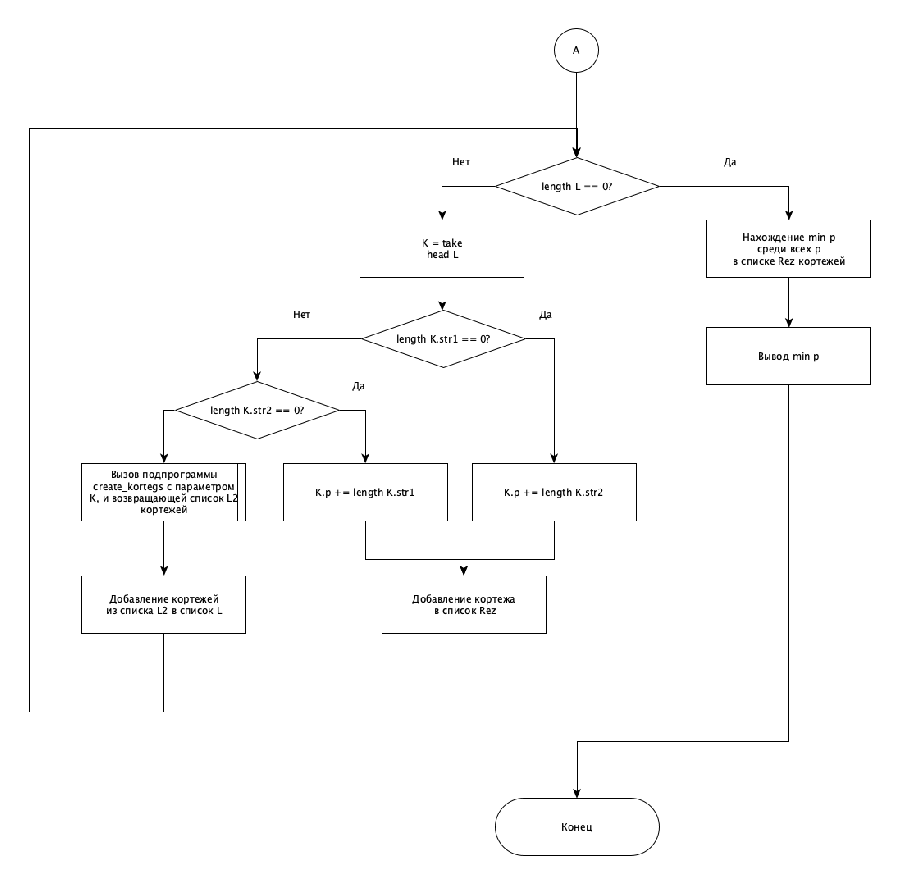
\includegraphics[width=1.6\linewidth]{LevenR_part2}
   \end{minipage}
   	\caption{Рекурсивная реализация.}
   	\label{ris:image1}
   \end{figure}

\newpage


	\begin{figure}[h!]
		\centering
		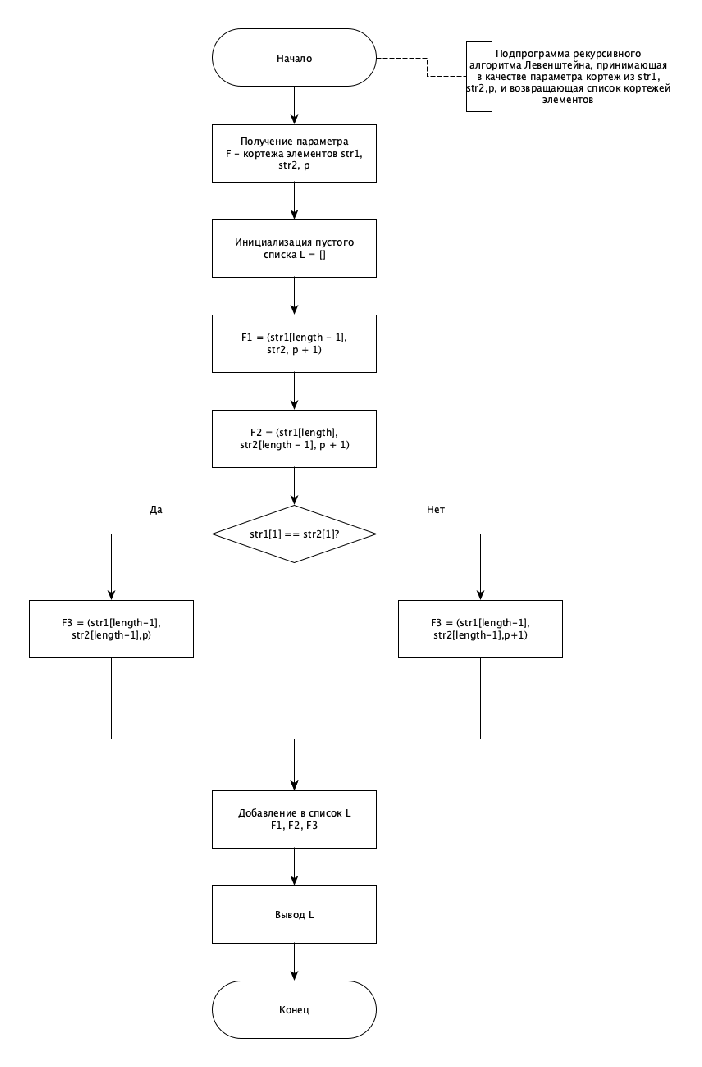
\includegraphics[width=0.7\linewidth]{LevenR_sub}
		\caption{Подпрограмма алгоритма Левенштейна.}
		\label{ris:image2}
	\end{figure}

\newpage
	
	\begin{figure}[h!]
		\centering
		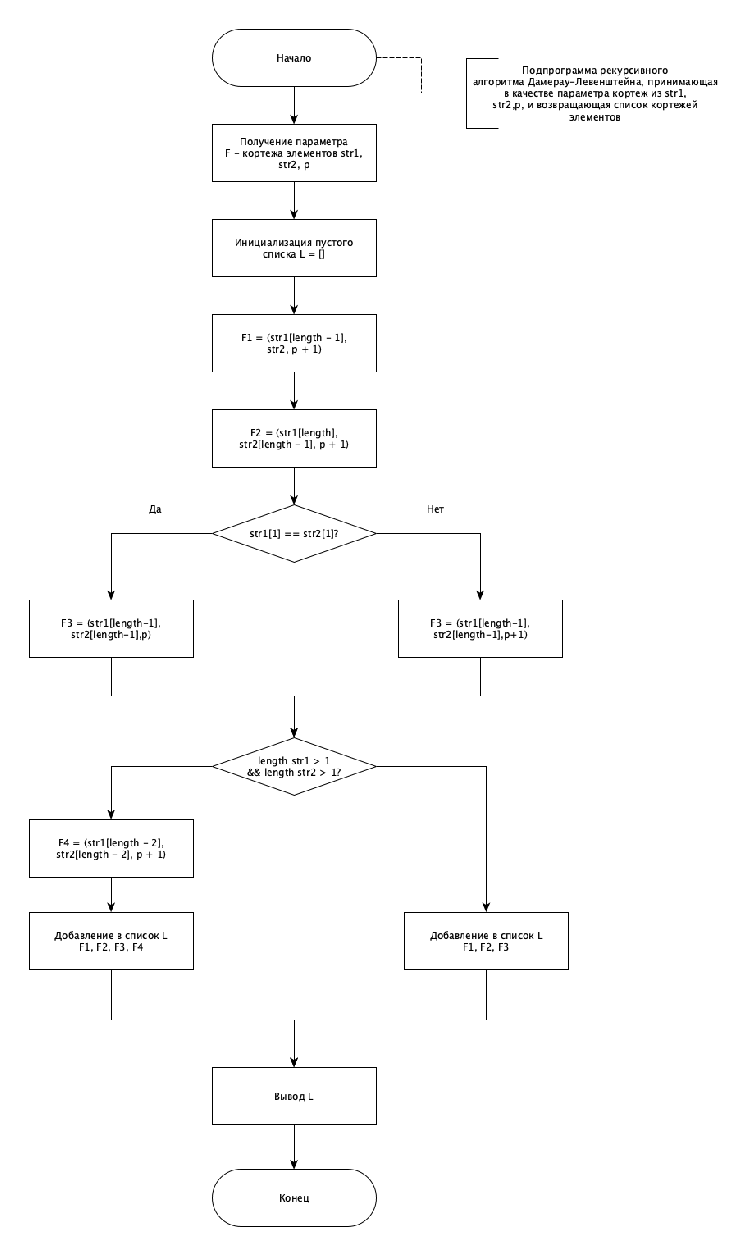
\includegraphics[width=0.7\linewidth]{LevenDomerauR}
		\caption{Подпрограмма алгоритма Дамерау-Левенштейна.}
		\label{ris:image3}
	\end{figure}
	
	\newpage
	
	\begin{figure}[h!]
		\centering
		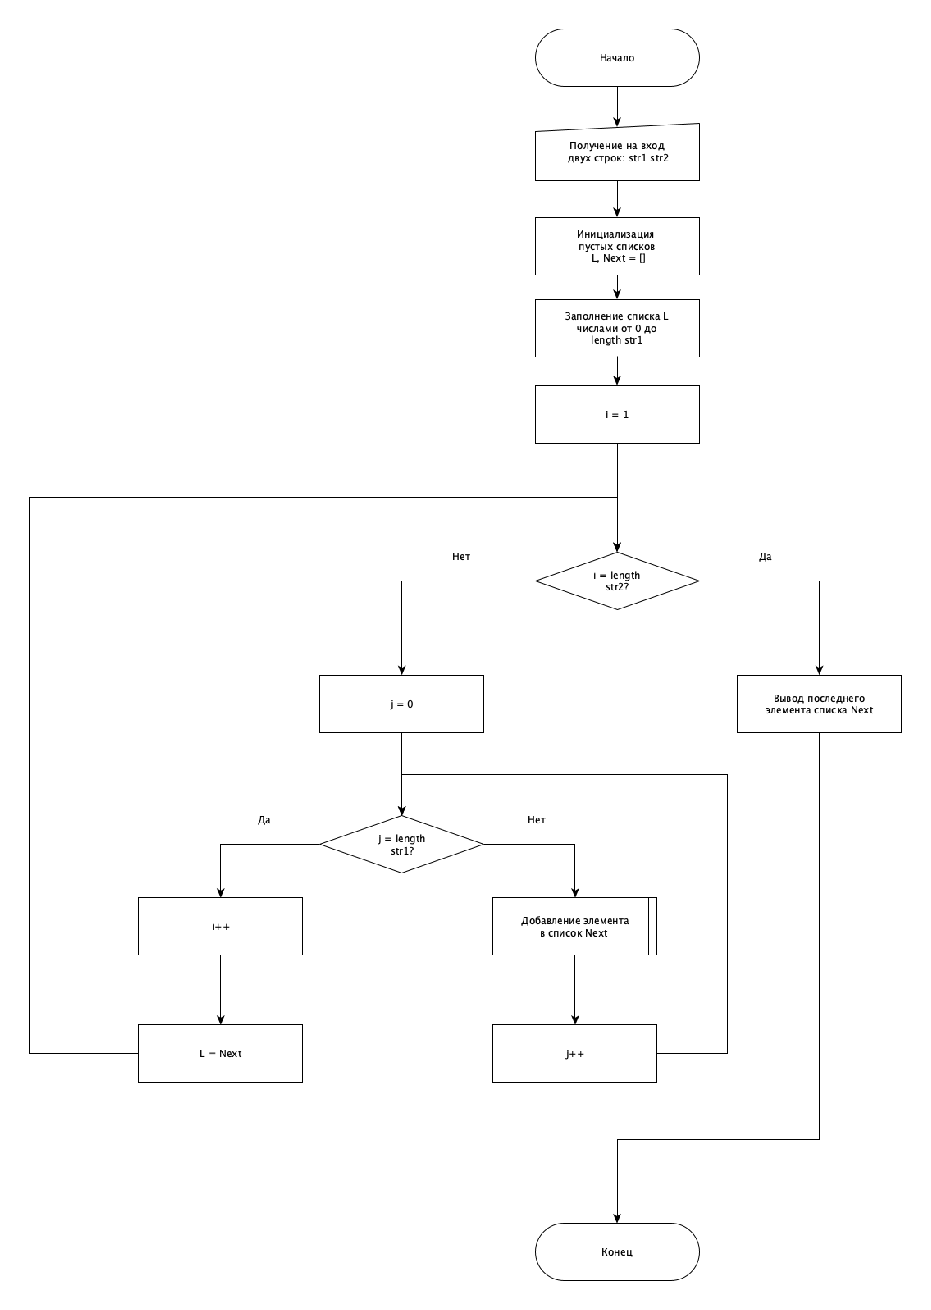
\includegraphics[width=0.9\linewidth]{LevenM}
		\caption{Матричный алгоритм Левенштейна.}
		\label{ris:image4}
	\end{figure}

\newpage
	
	\begin{figure}[h!]
		\centering
		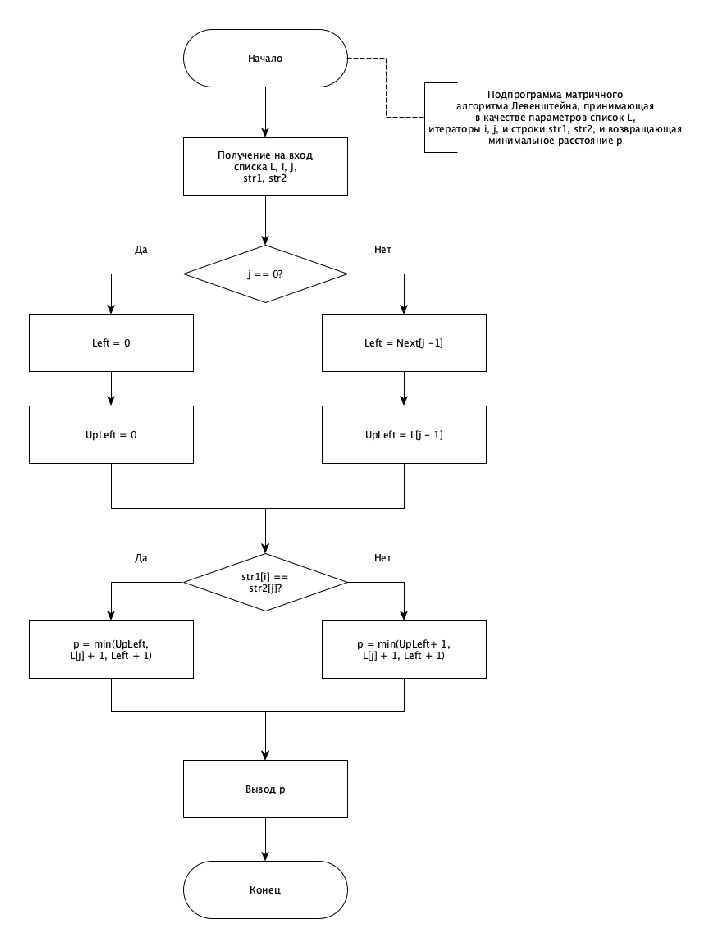
\includegraphics[width=0.8\linewidth]{LevenM_sub}
		\caption{Подпрограмма алгоритма Левенштейна.}
		\label{ris:image5}
	\end{figure}
	    
    \newpage
    
    \begin{figure}[h!]
    	\centering
    	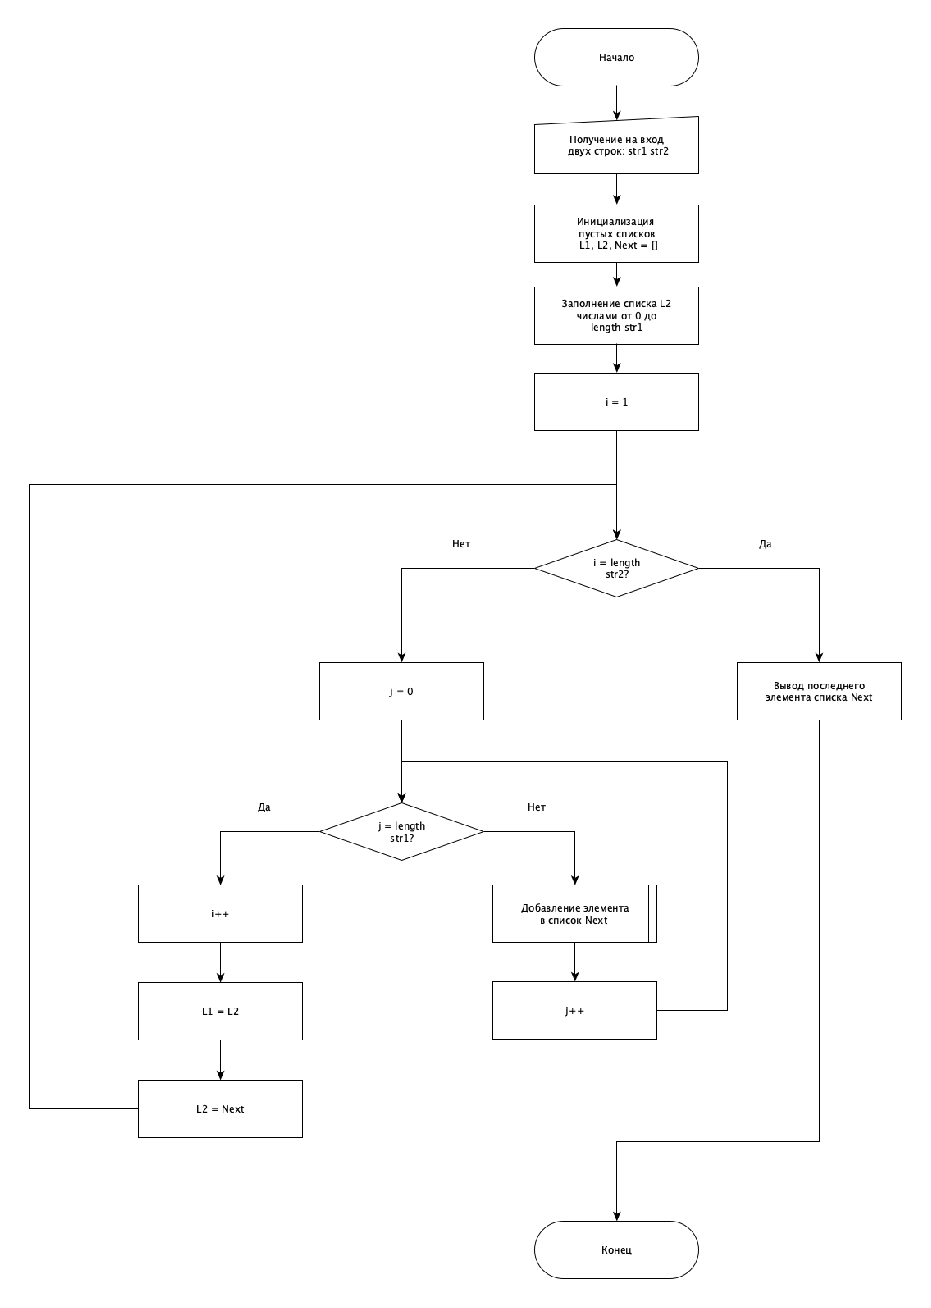
\includegraphics[width=0.8\linewidth]{LevenDomerauM}
    	\caption{Матричный алгоритм Дамерау-Левенштейна.}
    	\label{ris:image6}
    \end{figure}

\newpage

	\begin{figure}[h!]
		\centering
		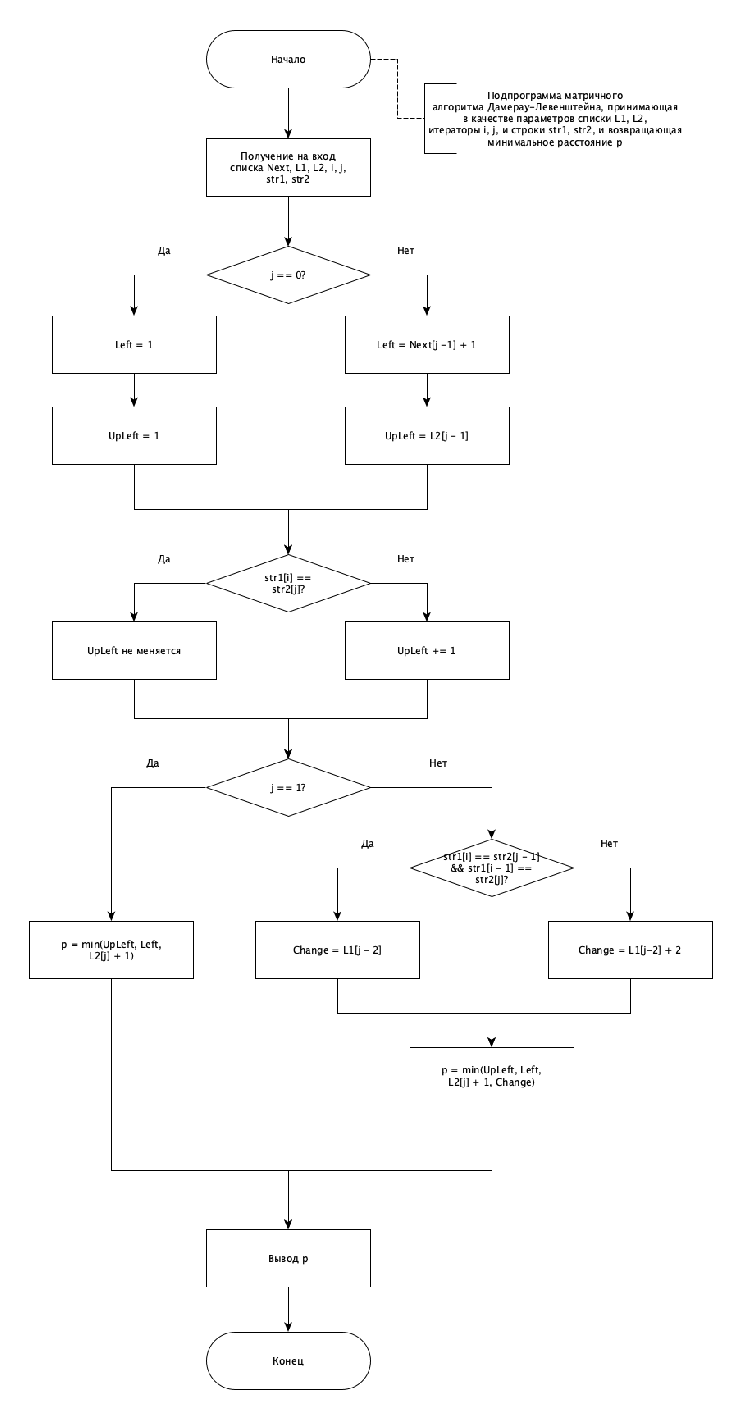
\includegraphics[width=0.6\linewidth]{LevenDomerauM_sub}
		\caption{Подпрограмма алгоритма Дамерау-Левенштейна.}
		\label{ris:image7}
	\end{figure}

    
    
    
    \section{Требования к программе}
    \begin{itemize}
    	\item Программа должна предоставлять доступный и понятный интерфейс с выбором алгоритмов (и всех их реализаций);
    	\item Должно быть 2 матричных реализации каждого алгоритма:
    	\begin{itemize}
    		\item хранит только те строки, которые необходимы для расчета последующих строк матрицы;
    		\item хранит всю матрицу целиком.
    	\end{itemize}
    	\item На вход каждой функции, реализующей конкретный алгоритм, подаются две строки латинского или русского алфавита;
    	\item Пользователь должен иметь возможность вводить строки вручную либо выбрать пункт случайного заполнения, в случае чего ему будет предоставлен выбор длины строк;
    	\item Uppercase и Lowercase буквы считаются разными;	
    	\item Требования к выводу программы:
	    \begin{itemize}
	    	\item программа должна выдавать корректное минимальное расстояние между двумя словами (см. Введение);
	    	\item при вводе пустых строк - программа не должна аварийно завершаться, а выдавать значение 0;
	    	\item помимо полученного значения, программа должна выдать процессорное время, затраченное на время выполнения данной реализации алгоритма;
	    	\item В случае выбора реализации матричного метода с запоминанием всей матрицы одного из алгоритмов, программа должна вывести на экран матрицу целиком.
	    \end{itemize}
    \end{itemize}
    
    
    \section{Выводы}
    В результате проведенной работы было решено реализовать алгоритмы Левенштейна и Дамерау-Левенштейна рекурсивными и матричными способами; были разработаны схемы алгоритмов.
    
    \chapter{Технологическая часть}
    \section{Выбор ЯП}
    
    В качестве языка программирования был выбран {\bf Haskell}, так как он является чистым функциональным языком и хорошо подходит для реализации рекурсивных алгоритмов.
    ~\cite{Haskell}
    
    \section{Замер времени}
    
    Время работы алгоритмов было замерено с помощью функции {\bf getCPUTime} из библиотеки {\bf System.CPUTime}.
    
    
    
    \section{Сведения о модулях программы}
    Программа состоит из:
    \begin{itemize}
    	\item Main.hs - Главный файл программы, в котором располагается меню;
    	\item Lib.hs - файл с подключенными модулями реализаций алгоритмов;
    	\item Domerau\_Levenshtein.hs - Файл с реализацией рекурсивного алгоритма Дамерау-Левенштейна;
    	\item Levenshtein\_matrix.hs - Файл с реализацией матричного алгоритма Левенштейна;
    	\item Domerau\_Levenshtein\_matrix.hs - Файл с реализацией матричного алгоритма Дамерау-Левенштейна;
    	\item Output\_Levenshtein\_matrix.hs - Файл с реализацией матричного алгоритма Левенштейна с хранением полной матрицы;
    	\item Output\_Domerau\_Levenshtein\_matrix.hs - Файл с реализацией матричного алгоритма Дамерау-Левенштейна  с хранением полной матрицы;
    	\item Spec.hs - Файл с модульными тестами.
    \end{itemize}

	{\bf Ниже приведены листинги  ~\ref{some-code1}, ~\ref{some-code2}, ~\ref{some-code3}, ~\ref{some-code4}, ~\ref{some-code5} функций программы.}
	    
    \begin{lstlisting}[label=some-code1,caption=Функция нахождения расстояния Дамерау-Левенштейна рекурсивно]
    import Data.List

    f ([],         [],         k) = [k]
    f (xs,         [],         k) = [k + length xs]
    f ([],         ys,         k) = [k + length ys]
    f (xs@(x:xs'), ys@(y:ys'), k) | ((xs' /= []) && (ys' /= [])) =
    calc_list $ (xs', ys, k + 1)
    : (xs, ys', k + 1) 
    : (xs', ys', k + if x == y then 0 else 1) 
    : if ((x == head ys') && (y == head xs'))
    then [(tail xs', tail ys', k + 1)] else []
    | otherwise                    = 
    calc_list $ (xs', ys, k + 1) 
    : (xs, ys', k + 1)
    : [(xs', ys', k + if x == y then 0 else 1)]
    calc_list []     = []
    calc_list (x:xs) = f x ++ calc_list xs
    
    domerau_levenshtein s1 s2 = minimum $ calc_list [(s1, s2, 0)]
    \end{lstlisting}
    
    \begin{lstlisting}[label=some-code2,caption=Функция нахождения расстояния Левенштейна матрично]
    import Data.List
    
    levenshtein s1 s2 = last $ foldl (transform s1) 
    [0..length s1] s2
    where transform str xs@(x:xs') c = res where
    res = x + 1 : zipWith4 compute str xs xs' res
    compute c' x y z = minimum [y + 1
    , z + 1
    , x + if c' == c 
    then 0 else 1]
    \end{lstlisting}
    
    \begin{lstlisting}[label=some-code3,caption=Функция нахождения расстояния Дамерау-Левенштейна матрично]
    import Data.List
    
    
    second_elem (_,x,_) = x
    
    res str xs@(x : xs') p1  = (xs, result, p1)
    where result           = x + 1 : zipWith4 compute str xs xs' result
    compute c1 x y z = minimum [y + 1
    , z + 1
    , x + if c1 == p1 then 0 else 1]
    
    res' str xs@(x : xs') ys p1 p2  = (xs, x + 1 : result, p1)
    where result = (compute (head str) 
    (head xs) 
    (head xs') 
    (x + 1))
    : zipWith6 compute_2 
    (tail str) 
    str 
    (tail xs) 
    (tail xs') 
    result ys
    compute   c1 x  y z     = minimum [y + 1
    , z + 1
    , x + if c1 == p1
    then 0 else 1]
    compute_2 c1 c2 x y z k = minimum [y + 1
    , z + 1
    , x + if c1 == p1
    then 0 else 1
    , k + if 
    ((c1 == p2) && (c2 == p1))
    then 1 else 2]
    
    
    domerau_levenshtein s1 s2 = last $ second_elem (foldl (transform s1) 
    ([], [0..(length s1)], ' ') s2)
    where transform str 
    (ys, xs@(x : xs'), p2) 
    p1 | ys == []  = res str xs p1
    | otherwise = res' str xs ys p1 p2
    \end{lstlisting}
    
    \begin{lstlisting}[label=some-code4,caption=Функция нахождения расстояния Левенштейна матрично с хранением матрицы]
    import Data.List
    
    levenshtein s1 s2 = (last $ fst rezult, reverse $ snd rezult) where
    rezult = foldl (transform s1) (fill_list, [fill_list]) s2
    where fill_list = [0..length s1]
    transform str (xs@(x:xs'), ys) c = (res, res : ys) where
    res = x + 1 : zipWith4 compute str xs xs' res
    compute c' x y z = minimum [y + 1
    , z + 1
    , x + if c' == c
    then 0 else 1]
    \end{lstlisting}
    
    \begin{lstlisting}[label=some-code5,caption=Функция нахождения расстояния Дамерау-Левенштейна матрично с хранением матрицы]
    import Data.List
    
    
    second_elem (_,x,_) = x
    
    res str xs@(x : xs') p1 zs = (xs, (result, result : zs), p1)
    where result           = x + 1 : zipWith4 compute str xs xs' result
    compute c1 x y z = minimum [y + 1
    , z + 1
    , x + if c1 == p1 then 0 else 1]
    
    res' str xs@(x : xs') ys p1 p2 zs = (xs
    , (x + 1 : result
    , ((x + 1) : result) : zs)
    , p1)
    where result                  = (compute (head str) 
    (head xs)
    (head xs') 
    (x + 1)) 
    : zipWith6 compute_2 (tail str) 
    str 
    (tail xs) 
    (tail xs') 
    result ys
    compute c1 x y z        = minimum [y + 1
    , z + 1
    , x + if c1 == p1 then 0 else 1]
    compute_2 c1 c2 x y z k = minimum [y + 1
    , z + 1
    , x + if c1 == p1 then 0 else 1
    , k + if ((c1 == p2) && (c2 == p1))
    then 1 else 2]
    
    
    domerau_levenshtein s1 s2 = (last $ fst rezult, reverse $ snd rezult) where
    rezult = second_elem (foldl (transform s1) 
    ([], (fill_list, [fill_list]), ' ') 
    s2)
    where fill_list = [0..(length s1)]
    transform str 
    (ys, (xs@(x : xs'), zs), p2) 
    p1 | ys == []  = res str xs p1 zs
    | otherwise = res' str xs ys p1 p2 zs
    \end{lstlisting}
    
    \section{Тесты}
    Тестирование было организовано с помощью библиотеки  \textbf{TestHUnit}.
    Было создано две вариации тестов:
    В первой сравнивались результаты функции с реальным результатом.
    
    Во второй сравнивались реузультаты двух функций (рекурсивной и табличной).
    При сравнении результатов двух функций использовалась функция randomRs из библиотеки System.Random, которая генерирует случайную строку нужной длины.
    
    \begin{lstlisting}[label=randStr,caption=Функция генерации случайной строки длины 7]
    take 7 $ randomRs ('a', 'z') randGen
    \end{lstlisting}
    Где randGen - генератор , инициализированный ранее с помощью функции newStdGen.
    
    В таблицах представлены тесты всех пяти реализаций алгоритмов:
    \begin{itemize}
    	\item Рекурсивный алгоритм Дамерау-Левенштейна
    	\item Матричный алгоритм Левенштейна
    	\item Матричный алгоритм Дамерау-Левенштейна
    	\item Матричный алгоритм Левенштейна (с выводом матрицы)
    	\item Матричный алгоритм Дамерау-Левенштейна (с выводом матрицы)
    \end{itemize}

	{\bf Ниже приведены таблицы ~\ref{tab:test1}, ~\ref{tab:test2}, ~\ref{tab:test3}, ~\ref{tab:test4}, ~\ref{tab:test5} тестов алгоритмов.}

    \begin{table}
    	\caption{\label{tab:test1} Рекурсивный алгоритм Дамерау-Левенштейна.}
    	\begin{center}
    		\begin{tabular}{|p{2.5cm}|c|c|c|c|c|}
    			\hline
    			  Описание теста & \multicolumn{2}{|c|}{Ввод} & Ожидаемое & Вывод & Результат\\
    			\hline
    			& Строка №1 & Строка №2 & & & \\
    			\hline
			   Пустые строки & "\_" & "\_" & 0 & 0 & \checkmark\\
			   \hline
   			   Вторая строка пуста & "a" & "\_" & 1 & 1 & \checkmark\\
   			   \hline
			   Первая строка пуста & "\_" & "a" & 1 & 1 & \checkmark\\
			   \hline
			   Одинаковые строки & "equal" & "equal" & 0 & 0 & \checkmark\\
			   \hline
			   Входные строки в кириллице & "одинаковые" & "одинаковые" & 0 & 0 & \checkmark\\
			   \hline
			   Обычный случай & "usual" & "specul" & 5 & 5 & \checkmark\\
			   \hline
			   Случай с совпадением 1 символа & "usual" & "qswer" & 4 & 4 & \checkmark\\
			   \hline
			   Одна строка больше другой & "usual" & "moreusual" & 4 & 4 & \checkmark\\
			   \hline
			   Случай с перестановкой двух соседних символов & "mroesuua" & "moreusual" & 3 & 3 & \checkmark\\
			   \hline
    		\end{tabular}
    	\end{center}
    \end{table}



\begin{table}
	\caption{\label{tab:test2} Матричный алгоритм Левенштейна.}
	\begin{center}
		\begin{tabular}{|p{2.5cm}|c|c|c|c|c|}
			\hline
			Описание теста & \multicolumn{2}{|c|}{Ввод} & Ожидаемое & Вывод & Результат\\
			\hline
			& Строка №1 & Строка №2 & & & \\
			\hline
			Пустые строки & "\_" & "\_" & 0 & 0 & \checkmark\\
			\hline
			Вторая строка пуста & "a" & "\_" & 1 & 1 & \checkmark\\
			\hline
			Первая строка пуста & "\_" & "a" & 1 & 1 & \checkmark\\
			\hline
			Одинаковые строки & "equal" & "equal" & 0 & 0 & \checkmark\\
			\hline
			Входные строки в кириллице & "одинаковые" & "одинаковые" & 0 & 0 & \checkmark\\
			\hline
			Обычный случай & "usual" & "specul" & 5 & 5 & \checkmark\\
			\hline
			Случай с совпадением 1 символа & "usual" & "qswer" & 4 & 4 & \checkmark\\
			\hline
			Одна строка больше другой & "usual" & "moreusual" & 4 & 4 & \checkmark\\
			\hline
		\end{tabular}
	\end{center}
\end{table}



\begin{table}
	\caption{\label{tab:test3} Матричный алгоритм Домерау-Левенштейна.}
	\begin{center}
		\begin{tabular}{|p{2.5cm}|c|c|c|c|c|}
			\hline
			Описание теста & \multicolumn{2}{|c|}{Ввод} & Ожидаемое & Вывод & Результат\\
			\hline
			& Строка №1 & Строка №2 & & & \\
			\hline
			Пустые строки & "\_" & "\_" & 0 & 0 & \checkmark\\
			\hline
			Вторая строка пуста & "a" & "\_" & 1 & 1 & \checkmark\\
			\hline
			Первая строка пуста & "\_" & "a" & 1 & 1 & \checkmark\\
			\hline
			Одинаковые строки & "equal" & "equal" & 0 & 0 & \checkmark\\
			\hline
			Входные строки в кириллице & "одинаковые" & "одинаковые" & 0 & 0 & \checkmark\\
			\hline
			Обычный случай & "usual" & "specul" & 5 & 5 & \checkmark\\
			\hline
			Случай с совпадением 1 символа & "usual" & "qswer" & 4 & 4 & \checkmark\\
			\hline
			Одна строка больше другой & "usual" & "moreusual" & 4 & 4 & \checkmark\\
			\hline
			Случай с перестановкой двух соседних символов & "mroesuua" & "moreusual" & 3 & 3 & \checkmark\\
			\hline
		\end{tabular}
	\end{center}
\end{table}

\newpage

\begin{center}
\begin{longtable}[H]{|p{2cm}|p{1.5cm}|p{1.5cm}|p{4.7cm}|p{4.7cm}|c|}
	\caption{\label{tab:test4} Матричный алгоритм Левенштейна с выводом матрицы.}\\
	\hline
	Описание теста & \multicolumn{2}{|c|}{Ввод} & Ожидаемое & Вывод & Рез\\
	\hline
	& Строка №1 & Строка №2 & & & \\
	\hline
	Пустые строки & "\_" & "\_" & (0, $[[0]]$) & (0, $[[0]]$) & \checkmark\\
	\hline
	Вторая строка пуста & "a" & "\_" & (1, $[[0,1]]$) & (1, $[[0,1]]$) & \checkmark\\
	\hline
	Первая строка пуста & "\_" & "a" & (1, $[[0],[1]]$) & (1, $[[0],[1]]$) & \checkmark\\
	\hline
	Одинаковые строки & "equal" & "equal" & (0,[
	
	$[0,1,2,3,4,5]$
	$,[1,0,1,2,3,4]$
	$,[2,1,0,1,2,3]$
	$,[3,2,1,0,1,2]$
	$,[4,3,2,1,0,1]$
	$,[5,4,3,2,1,0]$
	]) & (0,[
	
	$[0,1,2,3,4,5]$
	$,[1,0,1,2,3,4]$
	$,[2,1,0,1,2,3]$
	$,[3,2,1,0,1,2]$
	$,[4,3,2,1,0,1]$
	$,[5,4,3,2,1,0]$
	]) & \checkmark\\
	\hline
	Входные строки в кириллице & "один
	аковые" & "один
	аковые" & (0,[
	
	$[0,1,2,3,4,5,6,7,8,9,10]$
	$,[1,0,1,2,3,4,5,6,7,8,9]$
	$,[2,1,0,1,2,3,4,5,6,7,8]$
	$,[3,2,1,0,1,2,3,4,5,6,7]$
	$,[4,3,2,1,0,1,2,3,4,5,6]$
	$,[5,4,3,2,1,0,1,2,3,4,5]$
	$,[6,5,4,3,2,1,0,1,2,3,4]$
	$,[7,6,5,4,3,2,1,0,1,2,3]$
	$,[8,7,6,5,4,3,2,1,0,1,2]$
	$,[9,8,7,6,5,4,3,2,1,0,1]$
	$,[10,9,8,7,6,5,4,3,2,1,0]$
	]) & (0,[
	
	$[0,1,2,3,4,5,6,7,8,9,10]$
	$,[1,0,1,2,3,4,5,6,7,8,9]$
	$,[2,1,0,1,2,3,4,5,6,7,8]$
	$,[3,2,1,0,1,2,3,4,5,6,7]$
	$,[4,3,2,1,0,1,2,3,4,5,6]$
	$,[5,4,3,2,1,0,1,2,3,4,5]$
	$,[6,5,4,3,2,1,0,1,2,3,4]$
	$,[7,6,5,4,3,2,1,0,1,2,3]$
	$,[8,7,6,5,4,3,2,1,0,1,2]$
	$,[9,8,7,6,5,4,3,2,1,0,1]$
	$,[10,9,8,7,6,5,4,3,2,1,0]$
	]) & \checkmark\\
	\hline
	Обычный случай & "usual" & "specul" & (5,[
	
	$[0,1,2,3,4,5]$
	$,[1,1,1,2,3,4]$
	$,[2,2,2,2,3,4]$
	$,[3,3,3,3,3,4]$
	$,[4,4,4,4,4,4]$
	$,[5,4,5,4,5,5]$
	$,[6,5,5,5,5,5]$
	]) & (5,[
	
	$[0,1,2,3,4,5]$
	$,[1,1,1,2,3,4]$
	$,[2,2,2,2,3,4]$
	$,[3,3,3,3,3,4]$
	$,[4,4,4,4,4,4]$
	$,[5,4,5,4,5,5]$
	$,[6,5,5,5,5,5]$
	]) & \checkmark\\
	\hline
	Случай с совпадением 1 символа & "usual" & "qswer" & (4,[
	
	$[0,1,2,3,4,5]$
	$,[1,1,2,3,4,5]$
	$,[2,2,1,2,3,4]$
	$,[3,3,2,2,3,4]$
	$,[4,4,3,3,3,4]$
	$,[5,5,4,4,4,4]$
	]) & (4,[
	
	$[0,1,2,3,4,5]$
	$,[1,1,2,3,4,5]$
	$,[2,2,1,2,3,4]$
	$,[3,3,2,2,3,4]$
	$,[4,4,3,3,3,4]$
	$,[5,5,4,4,4,4]$
	]) & \checkmark\\
	\hline
	Одна строка больше другой & "usual" & "more
	usual" & (4,[
	
	$[0,1,2,3,4,5]$
	$,[1,1,2,3,4,5]$
	$,[2,2,2,3,4,5]$
	$,[3,3,3,3,4,5]$
	$,[4,4,4,4,4,5]$
	$,[5,4,5,4,5,5]$
	$,[6,5,4,5,5,6]$
	$,[7,6,5,4,5,6]$
	$,[8,7,6,5,4,5]$
	$,[9,8,7,6,5,4]$
	]) & (4,[
	
	$[0,1,2,3,4,5]$
	$,[1,1,2,3,4,5]$
	$,[2,2,2,3,4,5]$
	$,[3,3,3,3,4,5]$
	$,[4,4,4,4,4,5]$
	$,[5,4,5,4,5,5]$
	$,[6,5,4,5,5,6]$
	$,[7,6,5,4,5,6]$
	$,[8,7,6,5,4,5]$
	$,[9,8,7,6,5,4]$
	]) & \checkmark\\
	\hline
\end{longtable}
\end{center}

\newpage

\begin{center}
	\begin{longtable}[H]{|p{2cm}|p{1.5cm}|p{1.5cm}|p{4.7cm}|p{4.7cm}|c|}
		\caption{\label{tab:test5} Матричный алгоритм Левенштейна с выводом матрицы.}\\
		\hline
		Описание теста & \multicolumn{2}{|c|}{Ввод} & Ожидаемое & Вывод & Рез\\
		\hline
		& Строка №1 & Строка №2 & & & \\
		\hline
		Пустые строки & "\_" & "\_" & (0, $[[0]]$) & (0, $[[0]]$) & \checkmark\\
		\hline
		Вторая строка пуста & "a" & "\_" & (1, $[[0,1]]$) & (1, $[[0,1]]$) & \checkmark\\
		\hline
		Первая строка пуста & "\_" & "a" & (1, $[[0],[1]]$) & (1, $[[0],[1]]$) & \checkmark\\
		\hline
		Одинаковые строки & "equal" & "equal" & (0,[
		
		$[0,1,2,3,4,5]$
		$,[1,0,1,2,3,4]$
		$,[2,1,0,1,2,3]$
		$,[3,2,1,0,1,2]$
		$,[4,3,2,1,0,1]$
		$,[5,4,3,2,1,0]$
		]) & (0,[
		
		$[0,1,2,3,4,5]$
		$,[1,0,1,2,3,4]$
		$,[2,1,0,1,2,3]$
		$,[3,2,1,0,1,2]$
		$,[4,3,2,1,0,1]$
		$,[5,4,3,2,1,0]$
		]) & \checkmark\\
		\hline
		Входные строки в кириллице & "один
		аковые" & "один
		аковые" & (0,[
		
		$[0,1,2,3,4,5,6,7,8,9,10]$
		$,[1,0,1,2,3,4,5,6,7,8,9]$
		$,[2,1,0,1,2,3,4,5,6,7,8]$
		$,[3,2,1,0,1,2,3,4,5,6,7]$
		$,[4,3,2,1,0,1,2,3,4,5,6]$
		$,[5,4,3,2,1,0,1,2,3,4,5]$
		$,[6,5,4,3,2,1,0,1,2,3,4]$
		$,[7,6,5,4,3,2,1,0,1,2,3]$
		$,[8,7,6,5,4,3,2,1,0,1,2]$
		$,[9,8,7,6,5,4,3,2,1,0,1]$
		$,[10,9,8,7,6,5,4,3,2,1,0]$
		]) & (0,[
		
		$[0,1,2,3,4,5,6,7,8,9,10]$
		$,[1,0,1,2,3,4,5,6,7,8,9]$
		$,[2,1,0,1,2,3,4,5,6,7,8]$
		$,[3,2,1,0,1,2,3,4,5,6,7]$
		$,[4,3,2,1,0,1,2,3,4,5,6]$
		$,[5,4,3,2,1,0,1,2,3,4,5]$
		$,[6,5,4,3,2,1,0,1,2,3,4]$
		$,[7,6,5,4,3,2,1,0,1,2,3]$
		$,[8,7,6,5,4,3,2,1,0,1,2]$
		$,[9,8,7,6,5,4,3,2,1,0,1]$
		$,[10,9,8,7,6,5,4,3,2,1,0]$
		]) & \checkmark\\
		\hline
		Обычный случай & "usual" & "specul" & (5,[
		
		$[0,1,2,3,4,5]$
		$,[1,1,1,2,3,4]$
		$,[2,2,2,2,3,4]$
		$,[3,3,3,3,3,4]$
		$,[4,4,4,4,4,4]$
		$,[5,4,5,4,5,5]$
		$,[6,5,5,5,5,5]$
		]) & (5,[
		
		$[0,1,2,3,4,5]$
		$,[1,1,1,2,3,4]$
		$,[2,2,2,2,3,4]$
		$,[3,3,3,3,3,4]$
		$,[4,4,4,4,4,4]$
		$,[5,4,5,4,5,5]$
		$,[6,5,5,5,5,5]$
		]) & \checkmark\\
		\hline
		Случай с совпадением 1 символа & "usual" & "qswer" & (4,[
		
		$[0,1,2,3,4,5]$
		$,[1,1,2,3,4,5]$
		$,[2,2,1,2,3,4]$
		$,[3,3,2,2,3,4]$
		$,[4,4,3,3,3,4]$
		$,[5,5,4,4,4,4]$
		]) & (4,[
		
		$[0,1,2,3,4,5]$
		$,[1,1,2,3,4,5]$
		$,[2,2,1,2,3,4]$
		$,[3,3,2,2,3,4]$
		$,[4,4,3,3,3,4]$
		$,[5,5,4,4,4,4]$
		]) & \checkmark\\
		\hline
		Одна строка больше другой & "usual" & "more
		usual" & (4,[
		
		$[0,1,2,3,4,5]$
		$,[1,1,2,3,4,5]$
		$,[2,2,2,3,4,5]$
		$,[3,3,3,3,4,5]$
		$,[4,4,4,4,4,5]$
		$,[5,4,5,4,5,5]$
		$,[6,5,4,5,5,6]$
		$,[7,6,5,4,5,6]$
		$,[8,7,6,5,4,5]$
		$,[9,8,7,6,5,4]$
		]) & (4,[
		
		$[0,1,2,3,4,5]$
		$,[1,1,2,3,4,5]$
		$,[2,2,2,3,4,5]$
		$,[3,3,3,3,4,5]$
		$,[4,4,4,4,4,5]$
		$,[5,4,5,4,5,5]$
		$,[6,5,4,5,5,6]$
		$,[7,6,5,4,5,6]$
		$,[8,7,6,5,4,5]$
		$,[9,8,7,6,5,4]$
		]) & \checkmark\\
		\hline
		Случай с перестановкой двух соседних символов & "mroe
		suua" & "more
		usual" & (3,[
		
		$[0,1,2,3,4,5,6,7,8]$
		$,[1,0,1,2,3,4,5,6,7]$
		$,[2,1,1,1,2,3,4,5,6]$
		$,[3,2,1,1,2,3,4,5,6]$
		$,[4,3,2,2,1,2,3,4,5]$
		$,[5,4,3,3,2,2,2,3,4]$
		$,[6,5,4,4,3,2,2,3,4]$
		$,[7,6,5,5,4,3,2,2,3]$
		$,[8,7,6,6,5,4,3,3,2]$
		$,[9,8,7,7,6,5,4,4,3]$
		]) & (3,[
		
		$[0,1,2,3,4,5,6,7,8]$
		$,[1,0,1,2,3,4,5,6,7]$
		$,[2,1,1,1,2,3,4,5,6]$
		$,[3,2,1,1,2,3,4,5,6]$
		$,[4,3,2,2,1,2,3,4,5]$
		$,[5,4,3,3,2,2,2,3,4]$
		$,[6,5,4,4,3,2,2,3,4]$
		$,[7,6,5,5,4,3,2,2,3]$
		$,[8,7,6,6,5,4,3,3,2]$
		$,[9,8,7,7,6,5,4,4,3]$
		]) & \checkmark\\
		\hline
	\end{longtable}
\end{center}


\section{Выводы}

\begin{itemize}
	\item Был выбран язык программирования Haskell для реализации поставленной задачи;
	\item Был найден способ (функция) замера процессорного времени на языке Haskell;
	\item Были написаны тесты к программе;
	\item Была написана программа, удовлетворяющая всем требованиям, поставленным в конструкторской части;
\end{itemize}
        
    \chapter{Исследовательская часть}
    
    \section{Замер времени}
    
    Был проведен замер времени работы каждого из алгоритмов.
    
   \begin{table}[h]
   	\caption{\label{tab:time1} Время работы алгоритмов. }
   	\begin{center}
   		\begin{tabular}{|c|c|c|c|}
    		\hline
    		len & DamLev(R), нc & DamLev(T), нс & Lev(T), нс \\ [0.5ex] 
    		\hline
    		3 & 0.05122 & 0.00666 & 0.0118\\
    		\hline
    		4 & 0.21172 & 0.01661 & 0.01653\\
    		\hline
    		5 & 0.82129 & 0.01867 & 0.01785\\
    		\hline
    		6 & 3.90051 & 0.0322 & 0.02913\\
    		\hline
    		7 & 21.88572 & 0.04306 & 0.03041\\
    		\hline
    		8 & 131.24082 & 0.04461 & 0.04229\\
    		\hline
    		9 & 789.49599 & 0.05559 & 0.04601\\
    		\hline
    	\end{tabular}
    \end{center}
\end{table}


\begin{table}[h]
	\caption{\label{tab:time2} Время работы алгоритмов. }
	\begin{center}
		\begin{tabular}{|c|c|c|c|}
			\hline
			len & DamLev(T), нс & Lev(T), нс \\ [0.5ex] 
			\hline
			10 & 0.07763 & 0.05143\\
			\hline
			20 & 0.25776 & 0.17495\\
			\hline
			30 & 0.5983 & 0.37773\\
			\hline
			40 & 1.39289 & 0.75407\\
			\hline
			60 & 4.85997 & 2.40581\\
			\hline
			80 & 13.00983 & 5.97663\\
			\hline
			100 & 24.0279 & 12.90033\\
			\hline
		\end{tabular}
	\end{center}
\end{table}
    Где len - длина слова (подразумевается что длины обоих слов одинаковы, это было сделано для удобства) , DamLev(R) - Время работы рекурсивного алгоритма Дамерау-Левенштейна, Lev(T) - Время работы матричного алгоритма Левенштейна, DamLev(T) - Время работы матричного алгоритма Дамерау-Левенштейна.
    
    Время работы представлено в наносекундах. Для получения более точного результата процессорное время считалось как сумма всех времен, потраченных на каждый эксперимент, деленная на их количество:
    \[
    	T = \frac{\sum T_i}{N}, i \in [1, N]
    \]
    Где количество измерений было решено сделать равным 100. Строки на каждой итерации были составлены генератором случаных символов.
    
    \begin{tikzpicture}
    
    \begin{axis}[
    axis lines = left,
    xlabel = {$len$, букв},
    ylabel = {$time$, нс},
    legend pos=north west,
    ymajorgrids=true
    ]
    \addplot[color=red] table[x index=0, y index=1] {DamLevR.dat};
    \addplot[color=green, mark=square] table[x index=0, y index=1] {DamLevT.dat};
    
    \addlegendentry{DamLevR}
    \addlegendentry{DamLevT}
    \end{axis}
    \end{tikzpicture}
    
    \begin{tikzpicture}
    
    \begin{axis}[
    axis lines = left,
    xlabel = {$len$, букв},
    ylabel = {$time$, нс},
    legend pos=north west,
    ymajorgrids=true
    ]
    \addplot[color=blue, mark=square] table[x index=0, y index=1] {LevT.dat};
    \addplot[color=green, mark=square] table[x index=0, y index=1] {DamLevT2.dat};
    
    \addlegendentry{LevT}
    \addlegendentry{DamLevT}
    \end{axis}
    \end{tikzpicture}
    
    
    \par
    
     \section{Выводы}
     
    Исходя из представленных графиков, можно сделать следующие выводы:
    \begin{itemize}
    	\item матричная реализация алгоритмов Дамерау-Левенштейна {\bf значительно} быстрее рекурсивной. Уже при длине слова равном 5 результат различается почти в 80 раз, и далее растет экспоненциально;
    	\item  на больших входных данных (длины слов равны 100) матричная реализация алгоритма Дамерау-Левенштейна начинает быть почти в 2 раза менее эффективной чем матричная реализация алгоритма Левенштейна.
    \end{itemize}
    
    Таким образом, рекурсивная реализация (как и ожидалось), оказалась абсолютно бесполезным решением для данной задачи. Матричная реализация эффективнее как по памяти, так и по времени на {\bf любых} (не считая пустых значений) входных данных.
    
    А матричная реализация алгоритма Дамерау-Левенштейна справляется с поставленной задачей значительно медленнее (почти в 2 раза медленнее) чем реализация алгоритма Левенштейна на больших входных данных. (длины слов по 100 букв)
    
    \chapter*{Заключение}
    \addcontentsline{toc}{chapter}{Заключение}
    
    В рамках данной работы были изучены различные {\bf алгоритмы нечеткого поиска}. А именно:
    \begin{itemize}
    	\item Алгоритм Левенштейна;
    	\item Алгоритм Дамерау-Левенштейна;
    \end{itemize}
    
    А также их реализации:
    \begin{itemize}
    	\item Рекурсивный;
    	\item Матричный;
    \end{itemize}

    Экспериментально было подтверждено, что рекурсивная реализация гораздо медленнее эффективна как по времени, так и по памяти. Уже при значениях входных данных больше 5, разница во времени составляет больше чем в 80 раз. Это обусловливается тем, что рекурсивная реализация на каждом этапе своей рекурсии разбивает задачу на более мелкие, при этом не контролируя возможность образования повторяющихся случаев.
    
    В то время как матричная реализация использует обычный итеративный подход, не требующий больших затрат по памяти. (для вычисления следующей строки нам достаточно запомнить только 1-2 предыдущие строки)
    
    Также, алгоритм Левенштейна оказался более эффективным как по времени, так и по памяти, нежели алгоритм Дамерау-Левенштейна. При проведении эксперимента над их матричными реализациями оказалось, что время, затраченное на выполнение поставленной задачи, на больших входных данных (порядка 100 букв в слове) различается почти в 2 раза. Что неудивительно, ведь алгоритм Дамерау-Левенштейна добавляет дополнительный функционал к алгоритму Левенштейна, который проверяет входное слово на наличие опечаток. (две соседние буквы поменялись местами, подробнее см. Аналит. часть)
    
    \begin{thebibliography}{}
	\bibitem{Haskell}  https://www.haskell.org/documentation/ - Документация Haskell
	\bibitem{Algorithms} http://repo.ssau.ru/bitstream/Informacionnye-tehnologii-i-nanotehnologii/Algoritm-nechetkogo-poiska-v-bazah-dannyh-i-ego-prakticheskaya-realizaciya-64172/1/paper - Алгоритмы нечеткого поиска
	\bibitem{leven} Двоичные коды с исправлением выпадений, вставок и замещений символов. Доклады Академий Наук СССР, 1965. В. И. Левенштейн.
	\bibitem{damerau} A technique for computer detection and correction of spelling errors. Damerau Fred J.
	\bibitem{recurs} Indexing methods for approximate dictionary searching. Journal of Experimental Algorithmics, 2011. L. M. Boytsov
	\end{thebibliography}
    
\end{document}